\documentclass[ignorenonframetext,compress]{beamer}
\setbeamertemplate{caption}[numbered]
\setbeamertemplate{caption label separator}{: }
\setbeamercolor{caption name}{fg=normal text.fg}
\beamertemplatenavigationsymbolsempty
\usepackage{lmodern}
\usepackage{amssymb,amsmath}
\usepackage{ifxetex,ifluatex}
\usepackage{fixltx2e} % provides \textsubscript
\ifnum 0\ifxetex 1\fi\ifluatex 1\fi=0 % if pdftex
\usepackage[T1]{fontenc}
\usepackage[utf8]{inputenc}
\else % if luatex or xelatex
\ifxetex
\usepackage{mathspec}
\else
\usepackage{fontspec}
\fi
\defaultfontfeatures{Ligatures=TeX,Scale=MatchLowercase}
\fi
\usetheme{Singapore}
% use upquote if available, for straight quotes in verbatim environments
\IfFileExists{upquote.sty}{\usepackage{upquote}}{}
% use microtype if available
\IfFileExists{microtype.sty}{%
\usepackage{microtype}
\UseMicrotypeSet[protrusion]{basicmath} % disable protrusion for tt fonts
}{}
\newif\ifbibliography
\usepackage{graphicx,grffile}
\makeatletter
\def\maxwidth{\ifdim\Gin@nat@width>\linewidth\linewidth\else\Gin@nat@width\fi}
\def\maxheight{\ifdim\Gin@nat@height>\textheight0.8\textheight\else\Gin@nat@height\fi}
\makeatother
% Scale images if necessary, so that they will not overflow the page
% margins by default, and it is still possible to overwrite the defaults
% using explicit options in \includegraphics[width, height, ...]{}
\setkeys{Gin}{width=\maxwidth,height=\maxheight,keepaspectratio}

% Prevent slide breaks in the middle of a paragraph:
\widowpenalties 1 10000
\raggedbottom

\AtBeginPart{
\let\insertpartnumber\relax
\let\partname\relax
\frame{\partpage}
}
\AtBeginSection{
\ifbibliography
\else
\let\insertsectionnumber\relax
\let\sectionname\relax
\frame{\sectionpage}
\fi
}
\AtBeginSubsection{
\let\insertsubsectionnumber\relax
\let\subsectionname\relax
\frame{\subsectionpage}
}

\setlength{\parindent}{0pt}
\setlength{\parskip}{6pt plus 2pt minus 1pt}
\setlength{\emergencystretch}{3em}  % prevent overfull lines
\providecommand{\tightlist}{%
\setlength{\itemsep}{0pt}\setlength{\parskip}{0pt}}
\setcounter{secnumdepth}{0}
\usepackage{graphicx}
\usepackage{array}
\usepackage{tabularx}                                             % table environment providing flexibility
\usepackage{caption}                                              % for creating captions  
\usepackage{longtable}                                            % allows tables to span multiple pages
\usepackage{rotating}                                             % allows for sideways tables
\usepackage{float}                                                % floating environments; may not need in rmarkdown
\usepackage{placeins}                                             % keeps floats from moving
\usepackage{indentfirst}                                          % indents first paragraph of a section
\usepackage{mdwtab}                                               % continued float multi-page figure
\usepackage{enumerate}                                            % create lists
\usepackage{hyperref}                                             % highlight cross references
\usepackage{enumitem}                                             % numbered lists
\usepackage{upquote}                                              % produce grave accent in latex
\usepackage{verbatim}                                             % produces verbatim results
\usepackage{fancyvrb}                                             % verbatim in a box
\usepackage{textcomp}                                             % fixes error with packages interfering
\usepackage{cmap}                                                 % fix mapping characters to unicode
\usepackage{appendixnumberbeamer}
\usepackage{lscape}

\setbeamersize{text margin left=0.1in}
\setbeamersize{text margin right=0.1in}

\definecolor{pageCol}{rgb}{0.5,0.5,1.0}

\usepackage{tikz}                                                   % used in background


\usebackgroundtemplate{
  \tikz[overlay,remember picture] 
  \node[opacity=0.3, at=(current page.south east),anchor=south east,inner sep=0pt] {
    
\includegraphics[height=0.5in]{noaalogo.jpg}};
}

\setbeamertemplate{footline}
{
  \begin{beamercolorbox}[wd=.05\paperwidth,ht=0ex,dp=0ex,left]{framenumber in head/foot}%
    \insertframenumber/\inserttotalframenumber
    
  \end{beamercolorbox}%
}
\setbeamercolor{footline}{fg=pageCol}


\newcounter{saveenumi}



%To get two columns
\def\begincols{\begin{columns}}
\def\begincol{\begin{column}}
\def\endcol{\end{column}}
\def\endcols{\end{columns}}

\title{California Scorpionfish 2017 Stock Assessment}
\author{Melissa H Monk\(^1\), \and Xi He\(^1\), \and John Budrick\(^2\)}
\institute{\(^1\)Southwest Fisheries Science Center \and \(^2\)California Department of Fish and Wildlife}
\date{STAR Panel meeing July 24-28, 2017}

\begin{document}
\frame{\titlepage}

\begin{frame}
\tableofcontents[hideallsubsections]
\end{frame}

\section{Background and Biology}\label{background-and-biology}

\begin{frame}{California scorpionfish (\emph{Scorpaena guttata})}

\begin{itemize} 
 \item[\checkmark] Distributed from central California to Punta Eugenia, Baja California Sur, Mexico 
 \item[\checkmark] Rarely observed north of Pt. Conception  
 \item[\checkmark] Observed from the intertidal to 600 ft,  preferred depth range from 20-450 ft  
 \item[\checkmark] Demersal, found over both hard and soft bottom  
 \item[\checkmark] Venomous dorsal, anal and pelvic spines
\end{itemize}

\centering
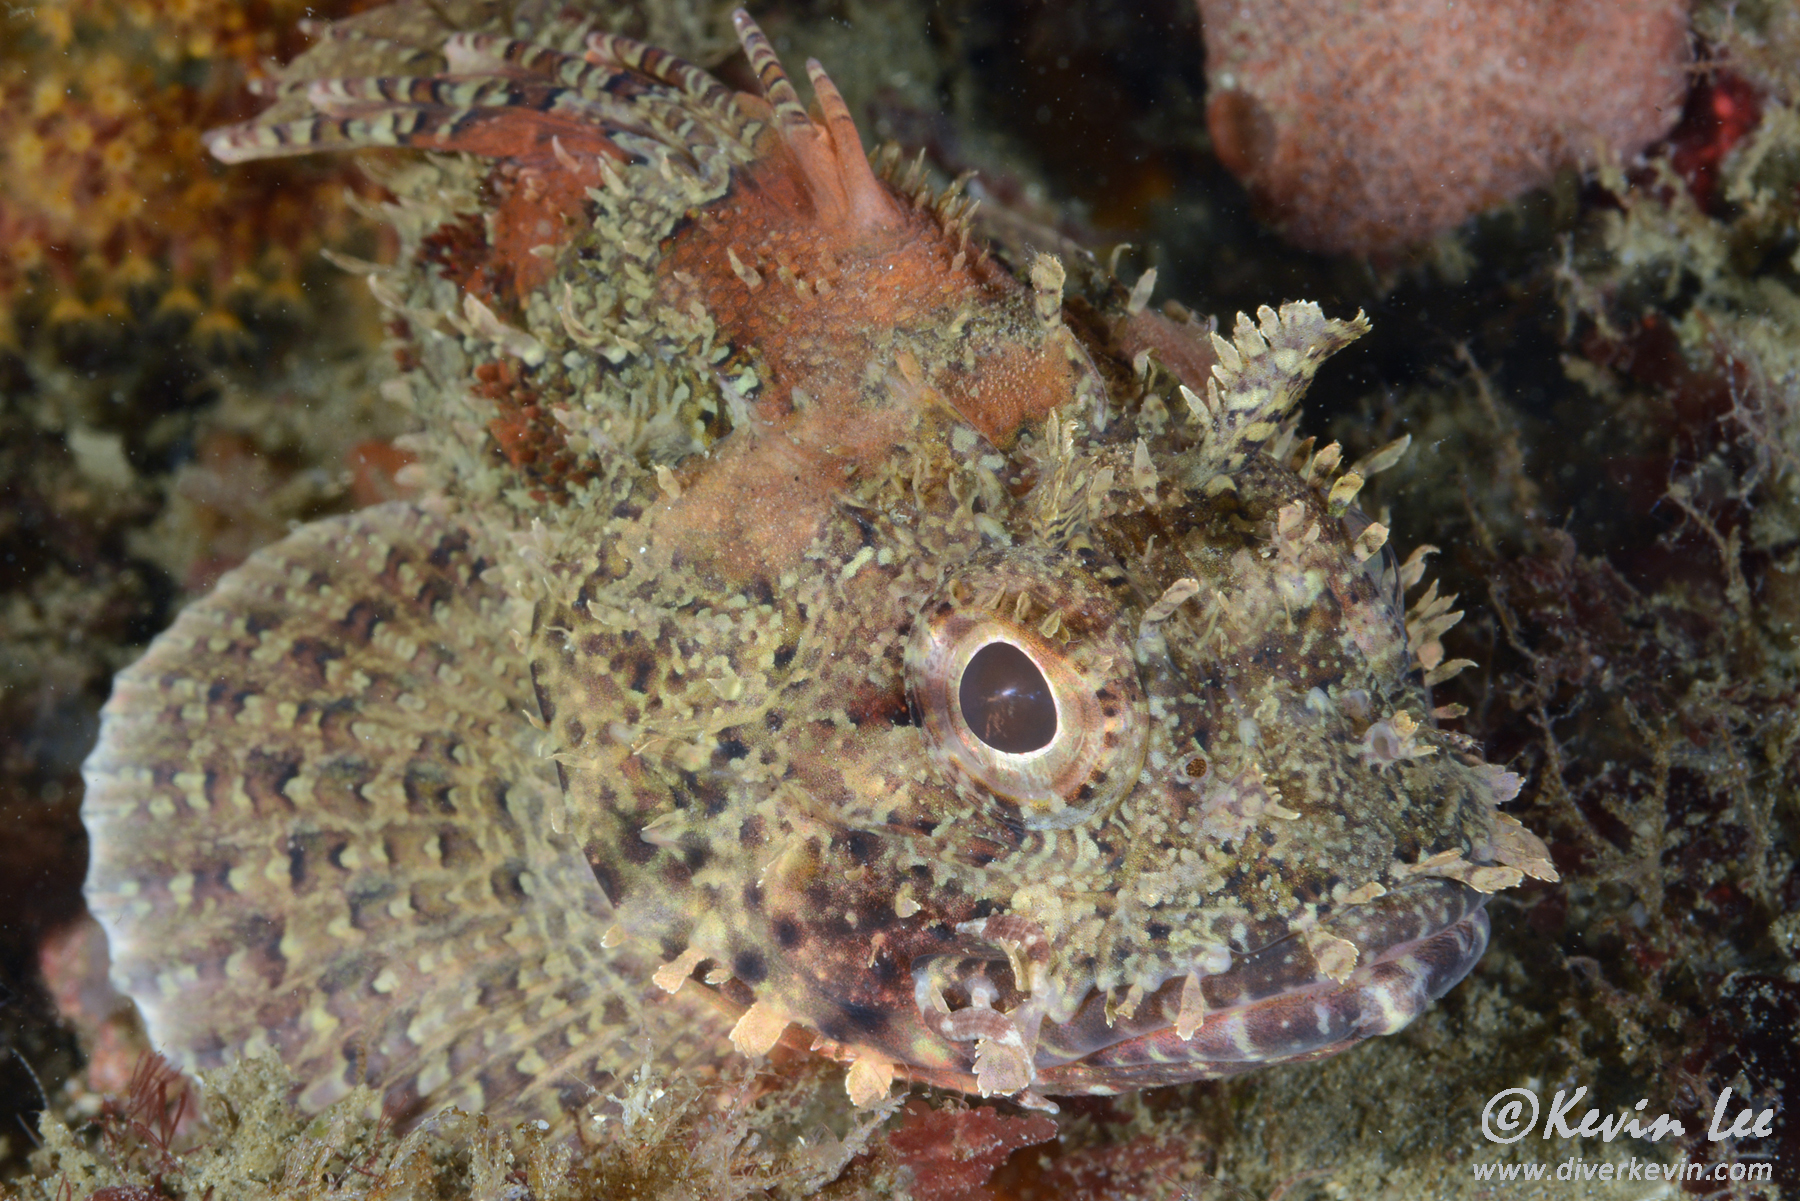
\includegraphics[width=.5\textwidth]{cover_photo}

\end{frame}

\begin{frame}{California scorpionfish (\emph{Scorpaena guttata})}

\begin{itemize} 
\item[\checkmark] Migration to spawning grounds, exhibit explosive breeding behavior just before dawn
\item[\checkmark] Exhibit aggregating behavior (spawning and non-spawning aggregations)  
\item[\checkmark] External fertilization, females produce eggs in a hollow gelaenous matrix
\item[\checkmark] Eggs hatch after about 5 days
\item[\checkmark] Juveniles settle at less than 2cm 
\end{itemize}

\centering
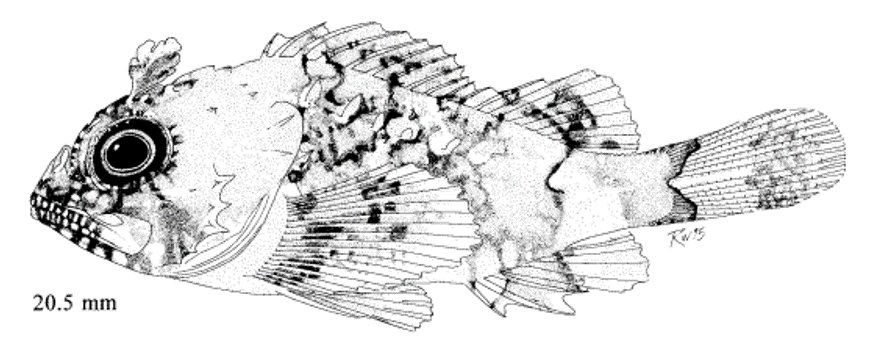
\includegraphics[width=.5\textwidth]{Figures/baby_scorp}

\footnotetext{Line drawning from CalCOFI Atlas 33, pg. 789 Figure 26}

\end{frame}

\subsection{Length-at-age}\label{length-at-age}

\begin{frame}{Length-at-age}

\begincols
 \begincol{.4\textwidth}

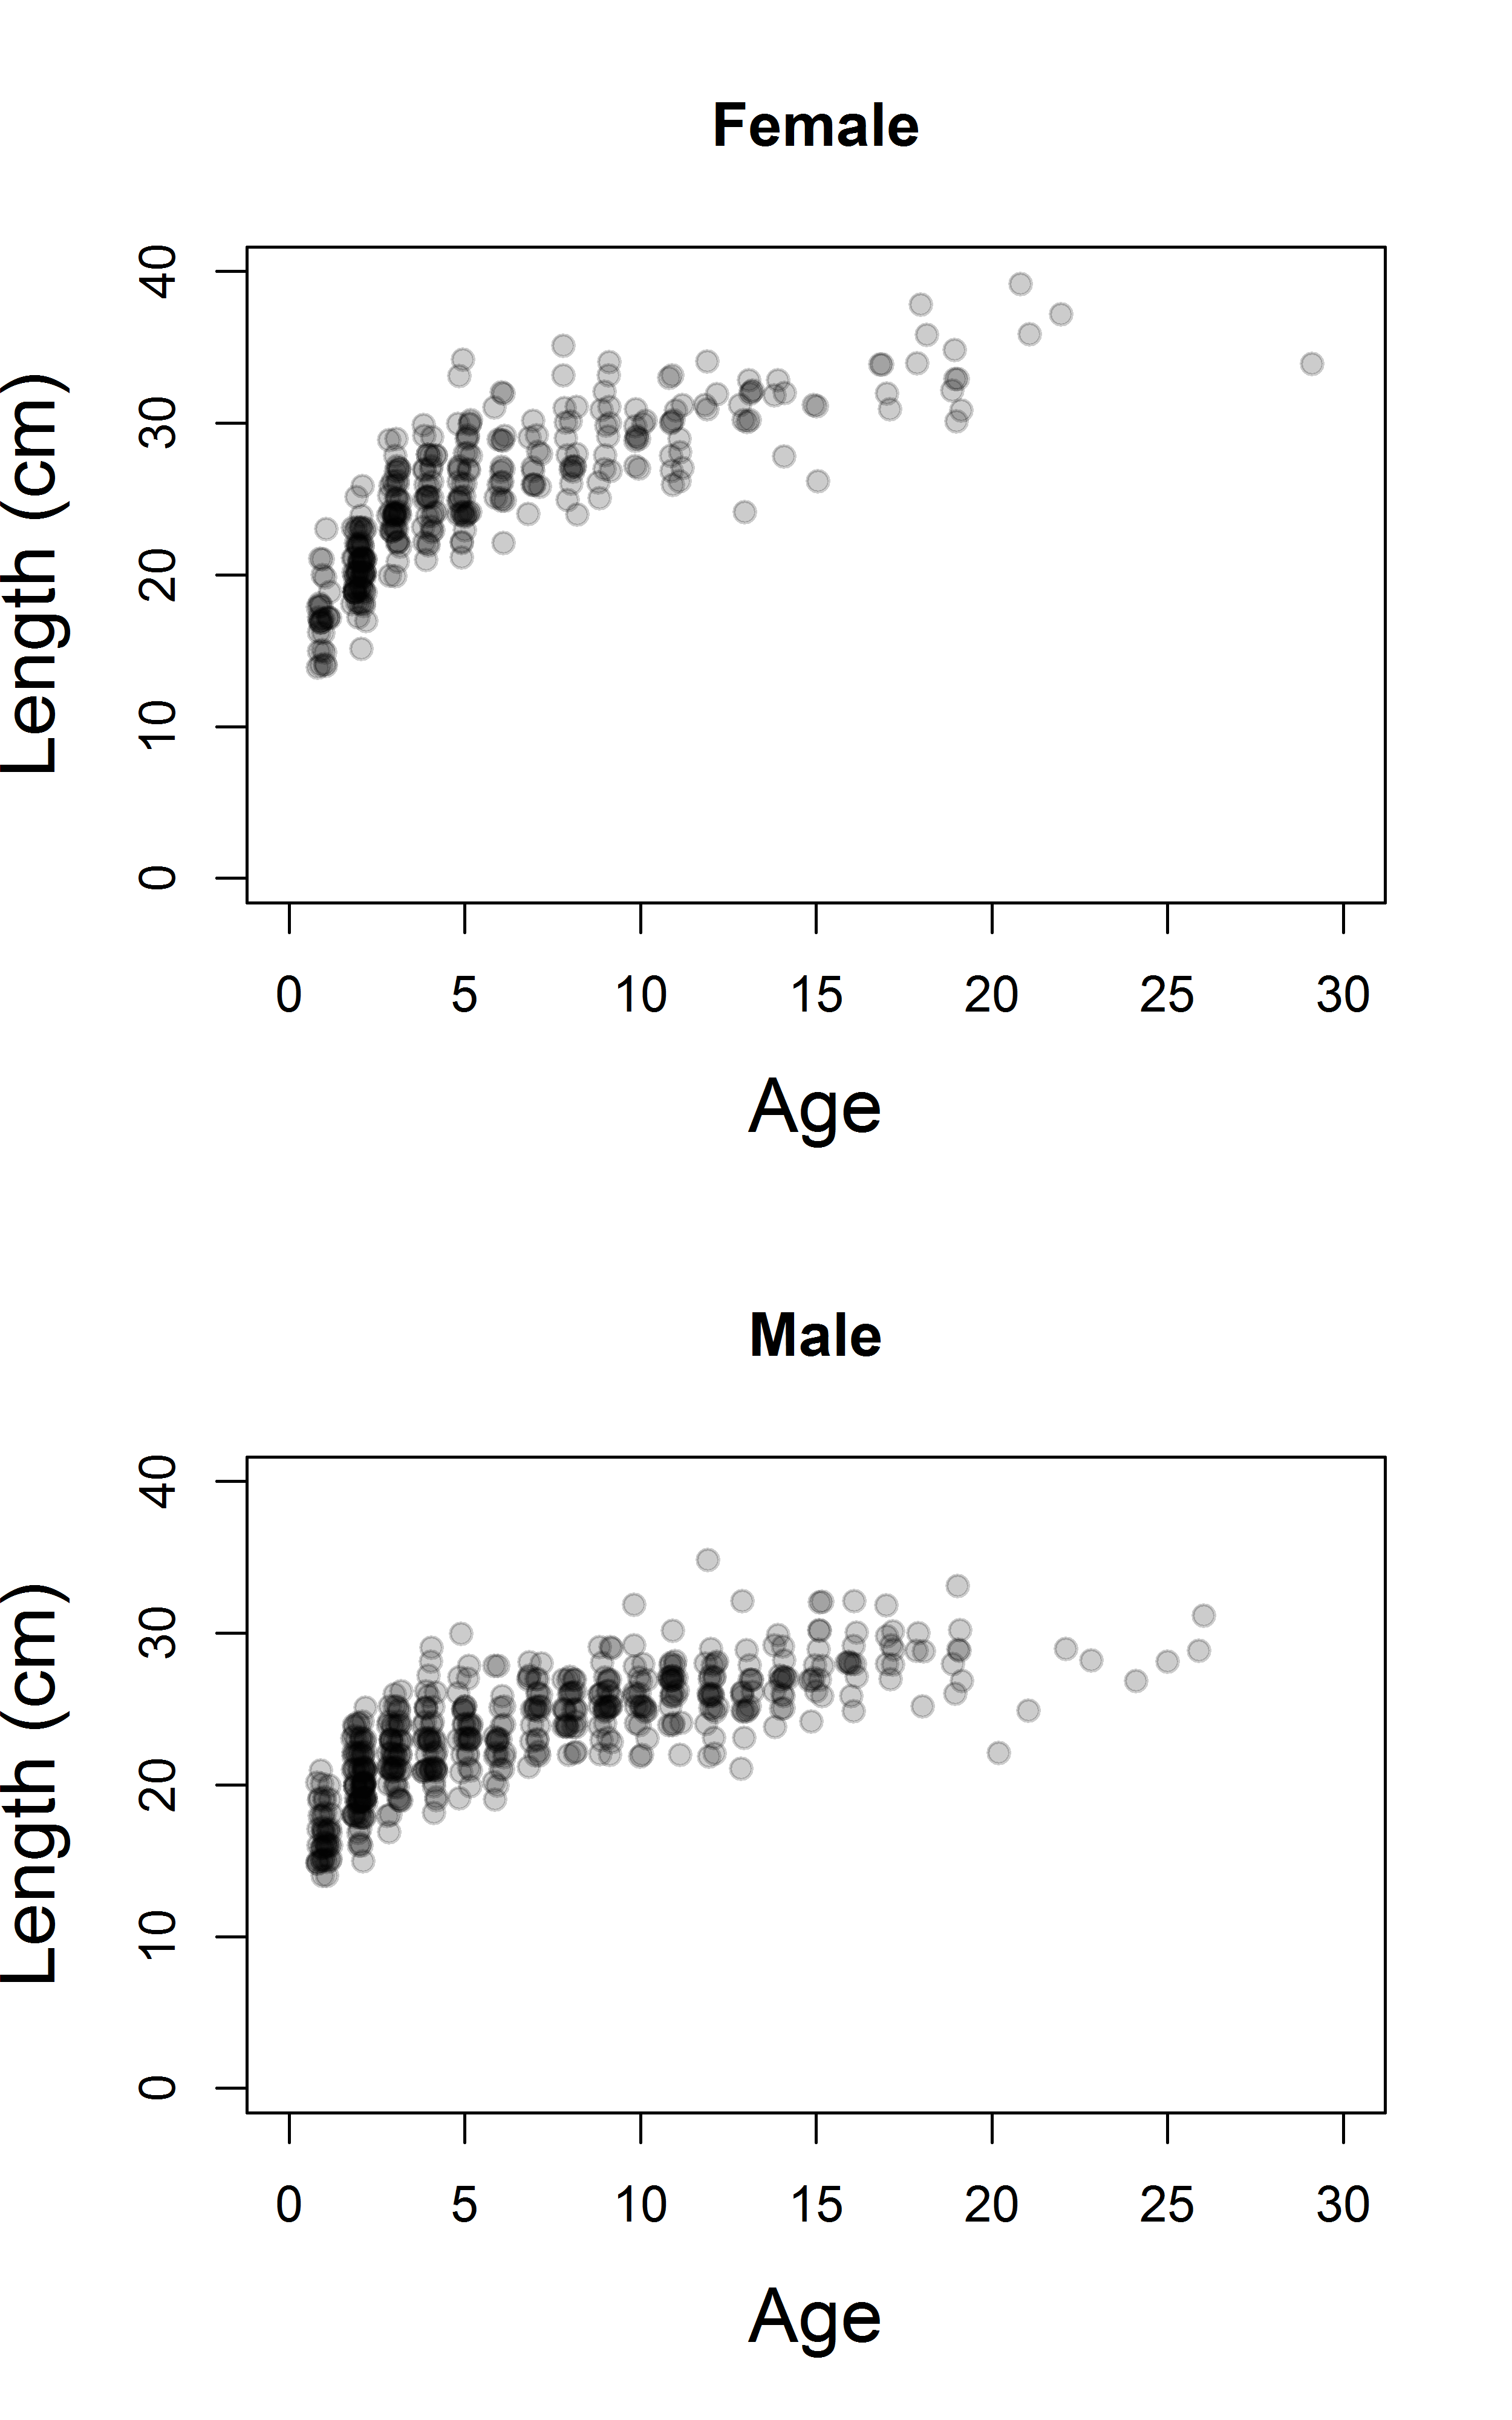
\includegraphics[trim={0 0 0 2cm}, totalheight=0.65\textheight]{Figures/Age_length_bySex.png}

\endcol
 \begincol{.48\textwidth}

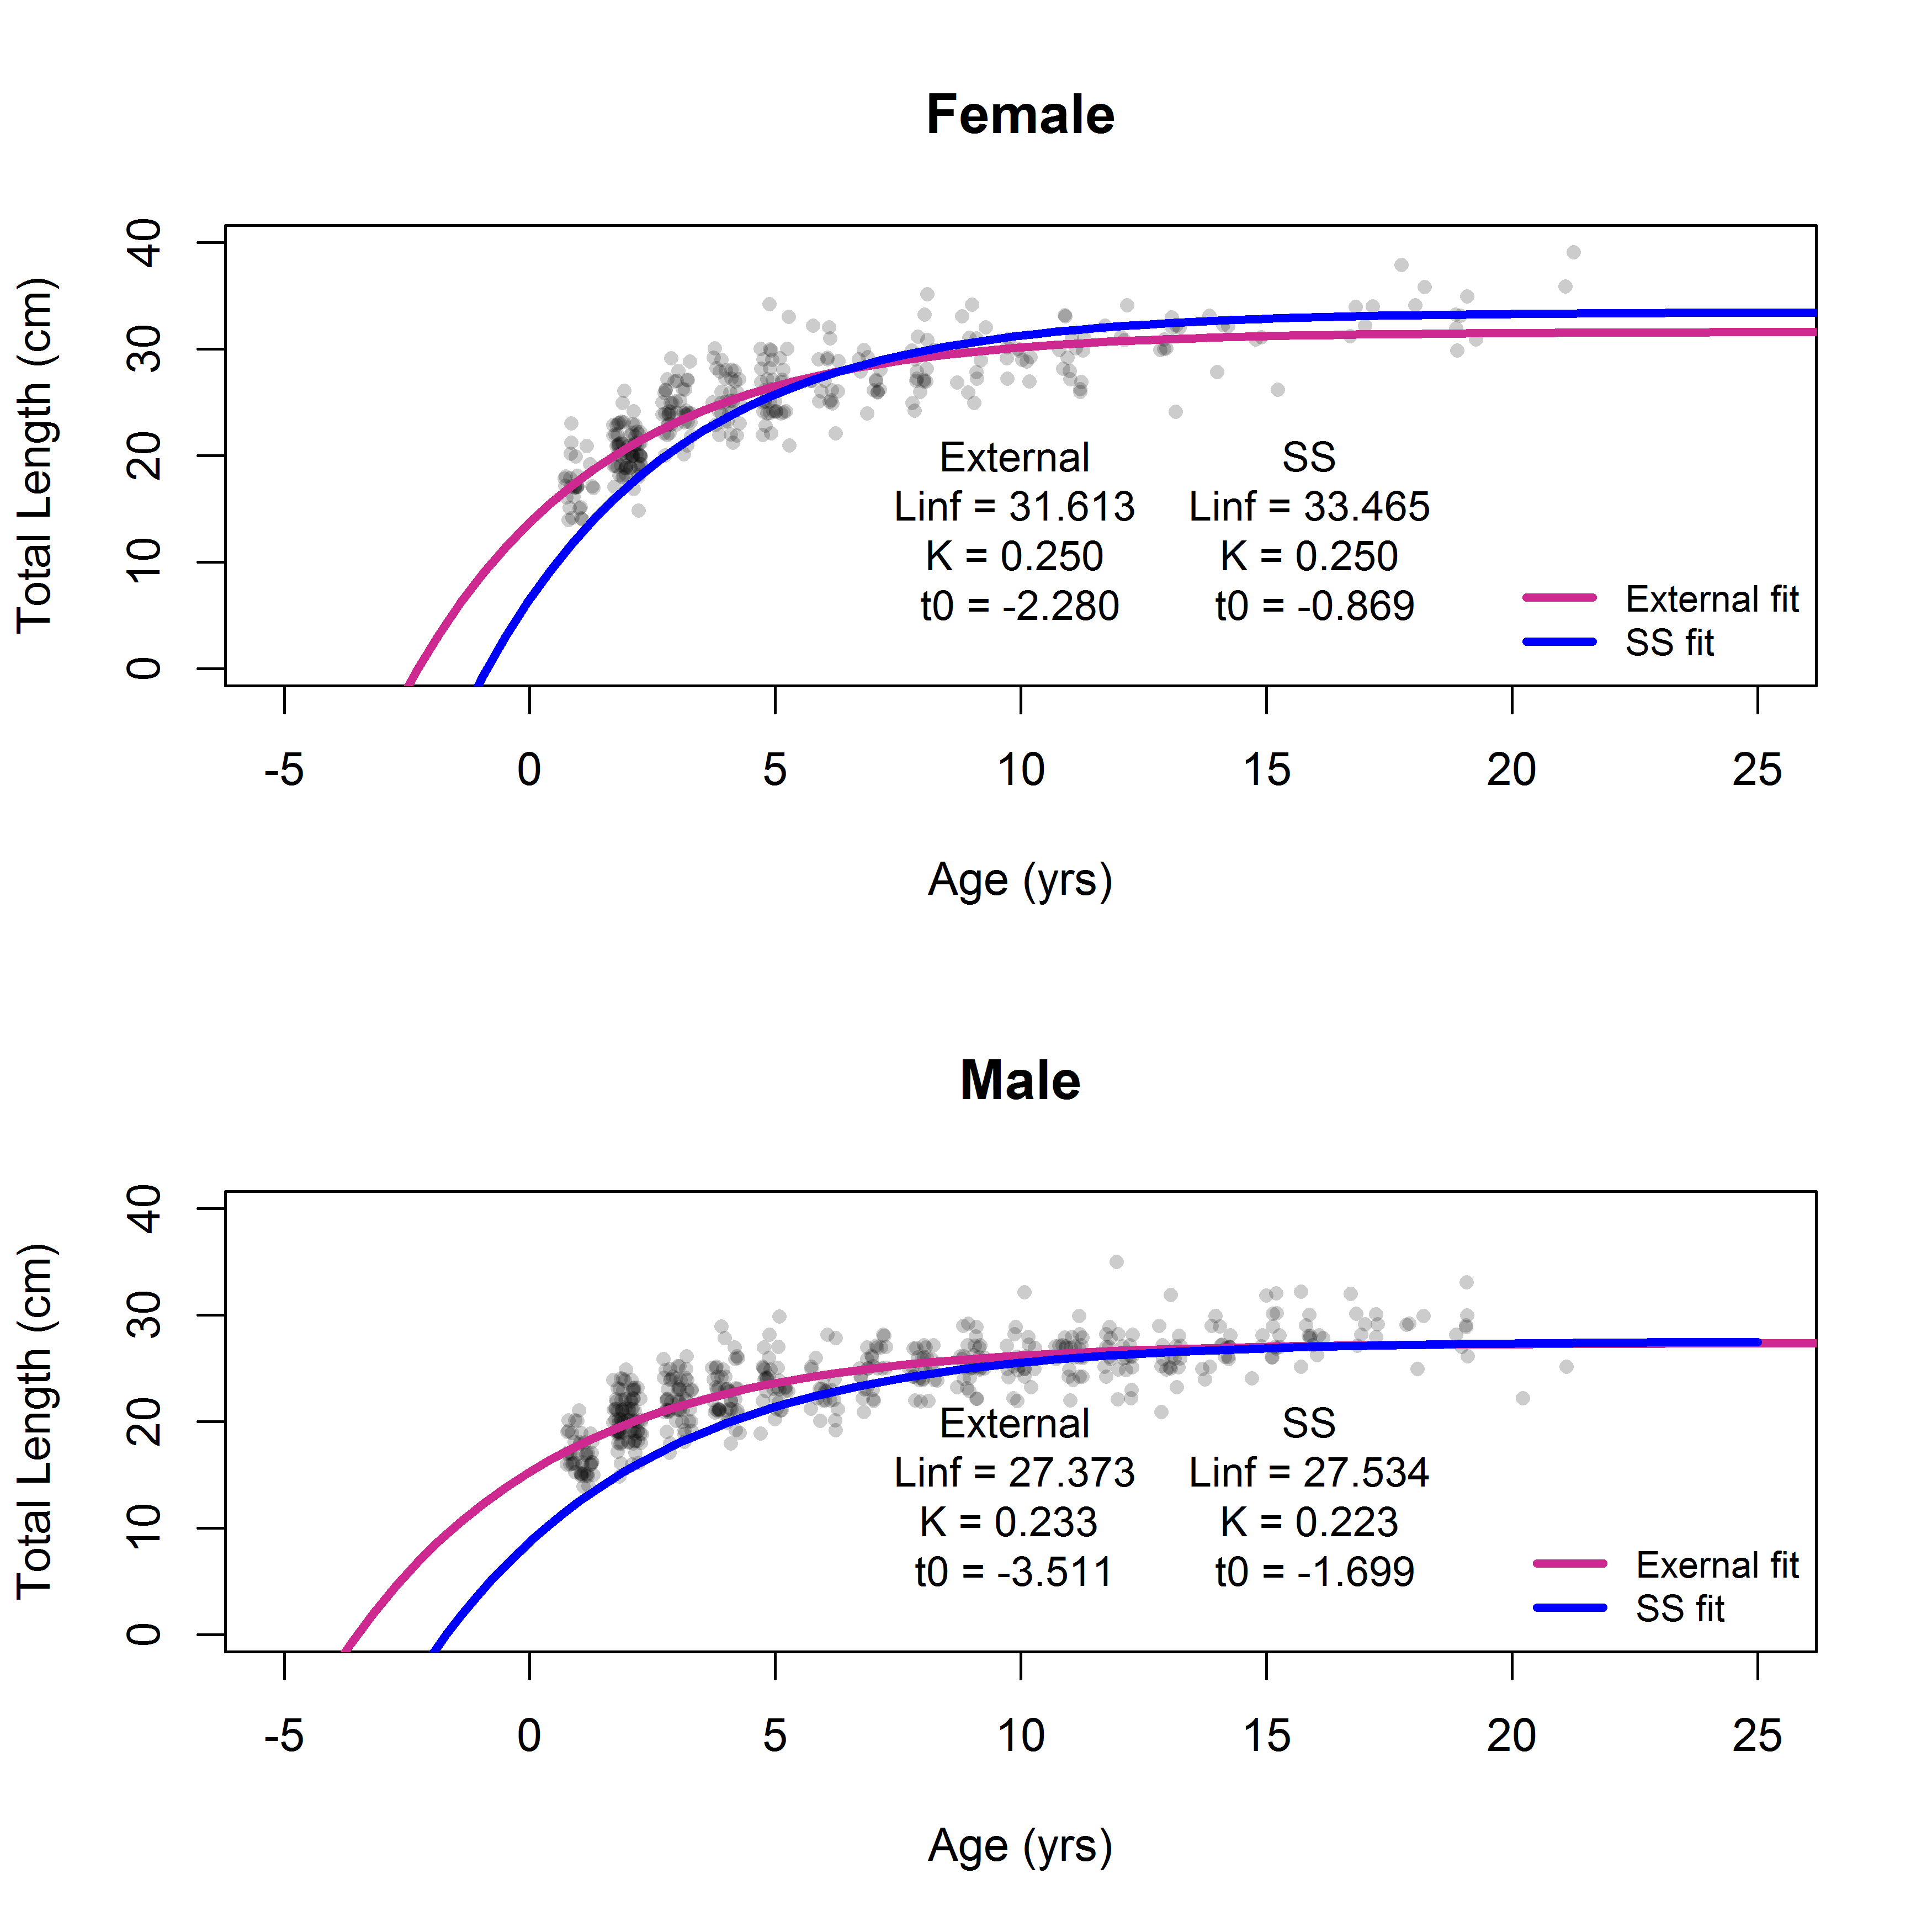
\includegraphics{Figures/vonB_compare.png}

\endcol
\endcols

\end{frame}

\begin{frame}{Length-at-age}

\begincols
 \begincol{.4\textwidth}

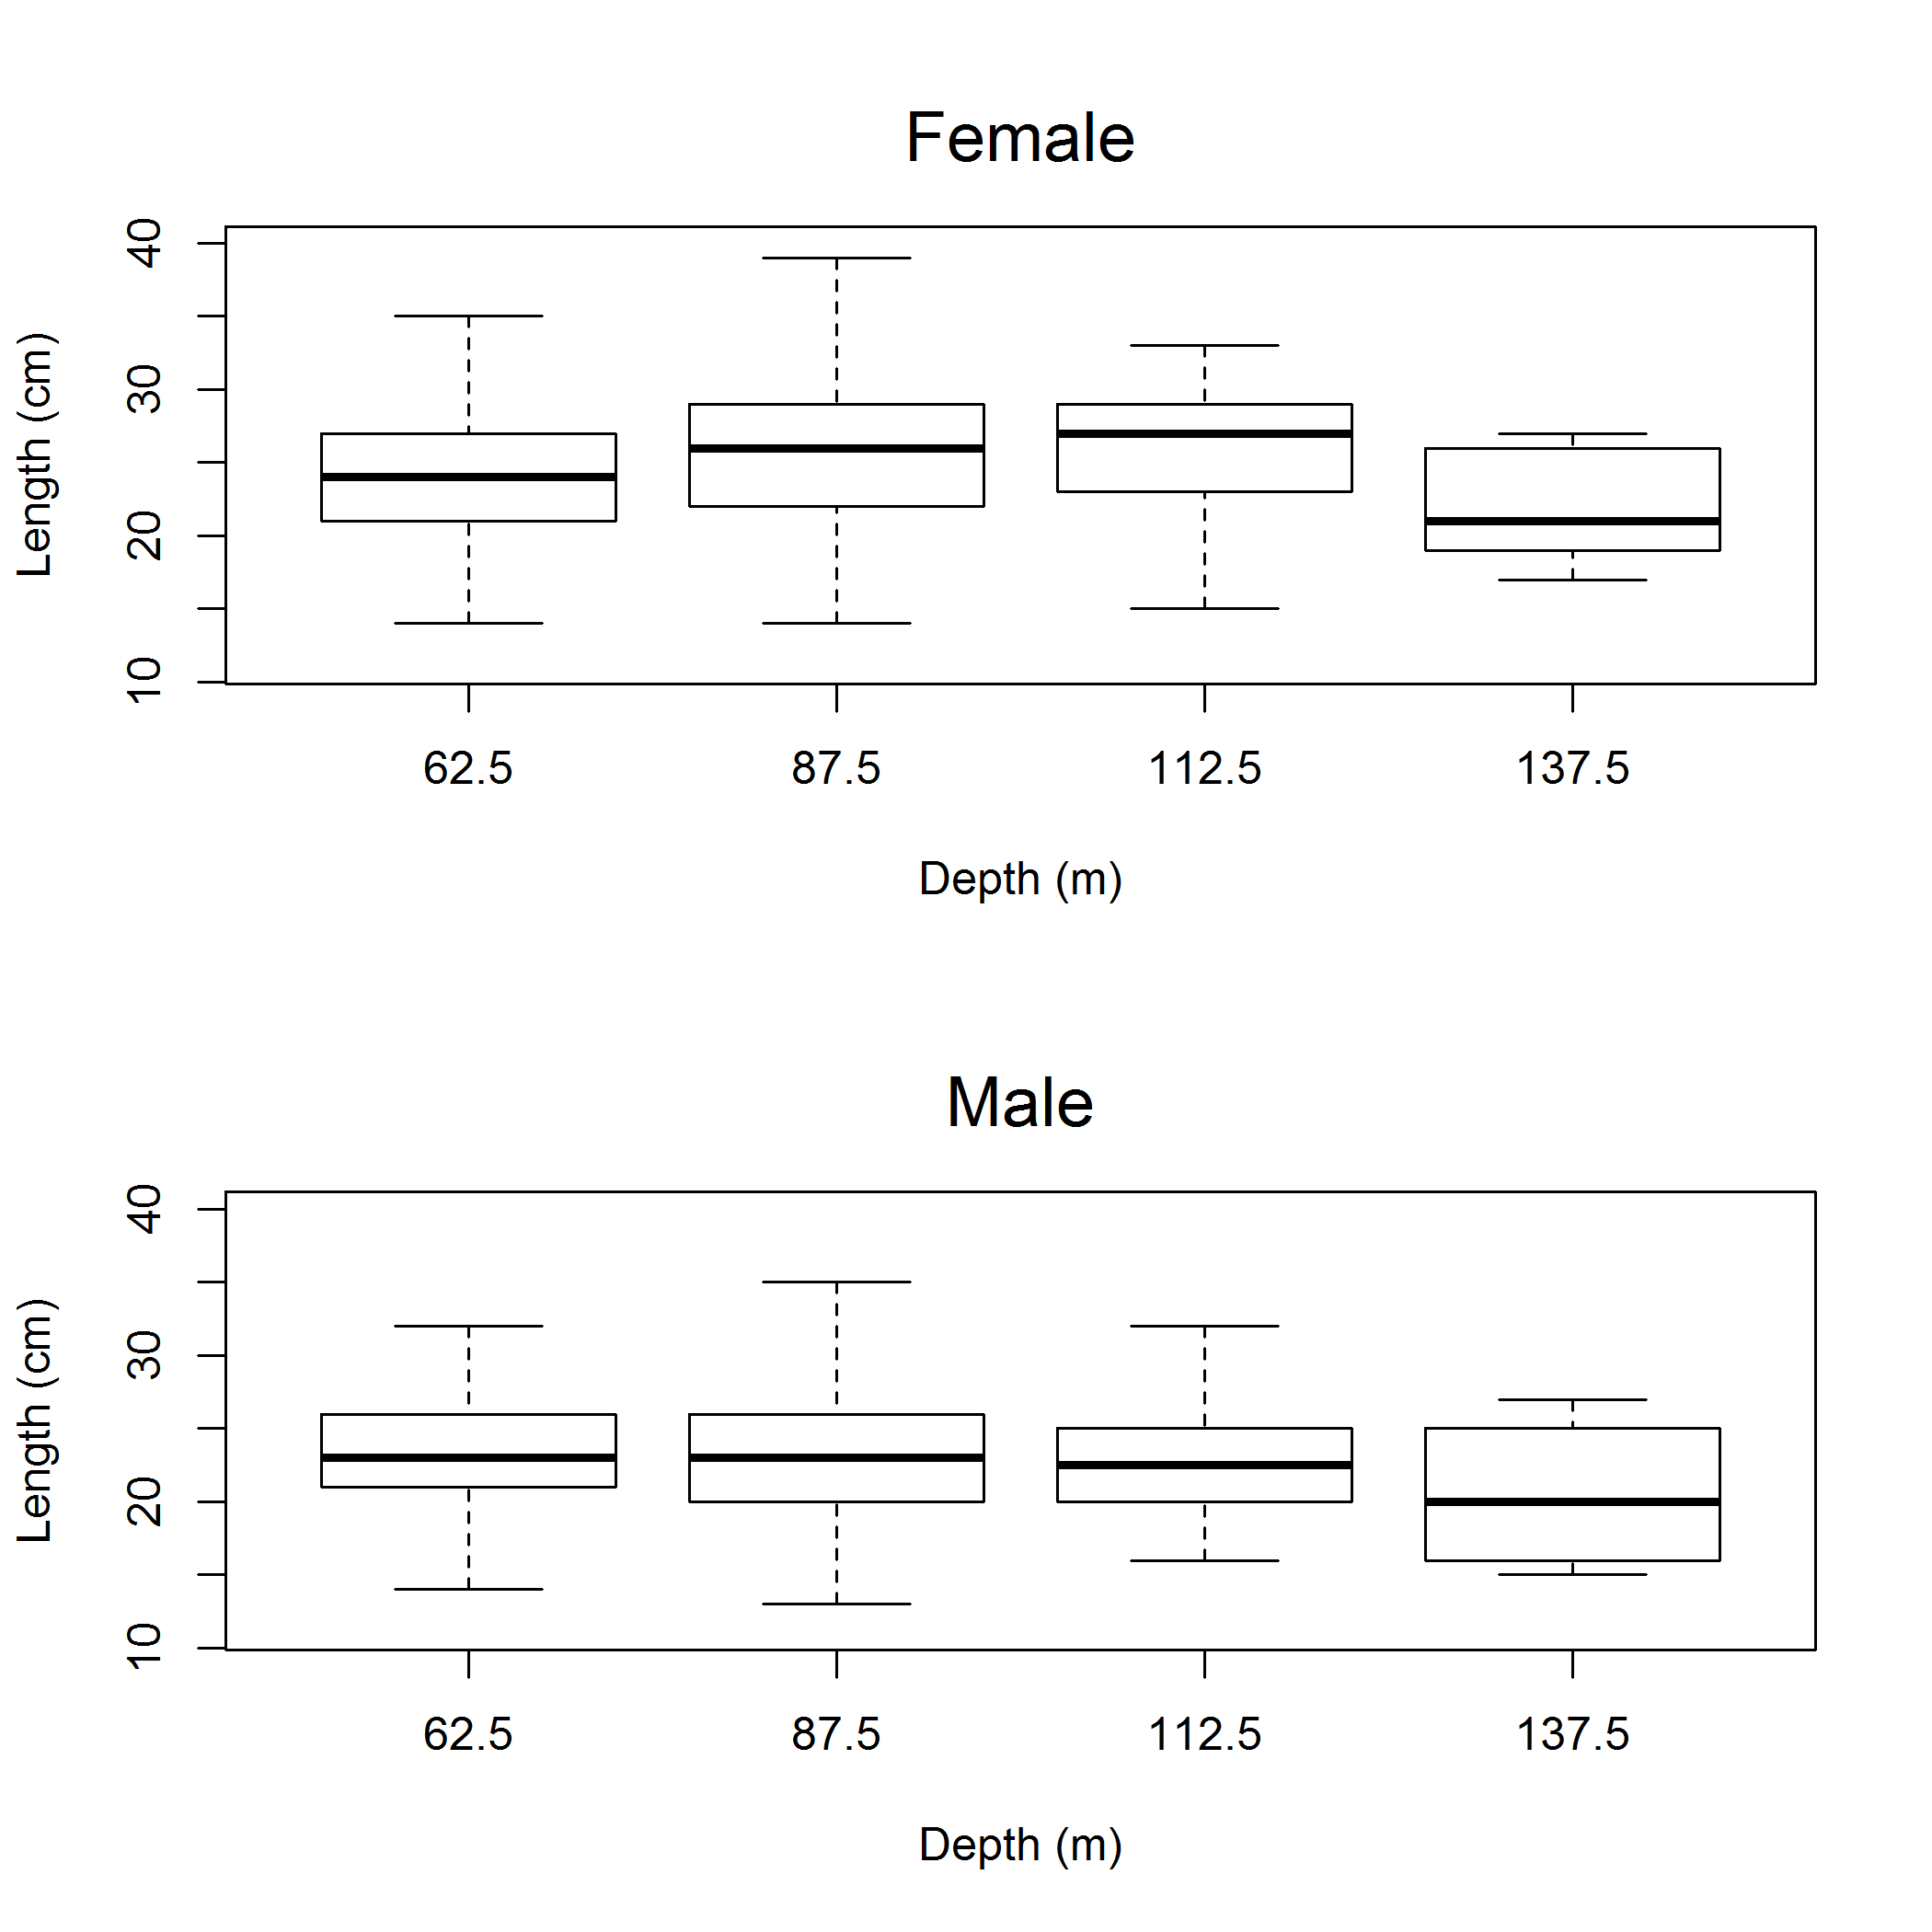
\includegraphics{Figures/NWFSCtrawl_lengthdepth.png}

\endcol
\begincol{.48\textwidth}

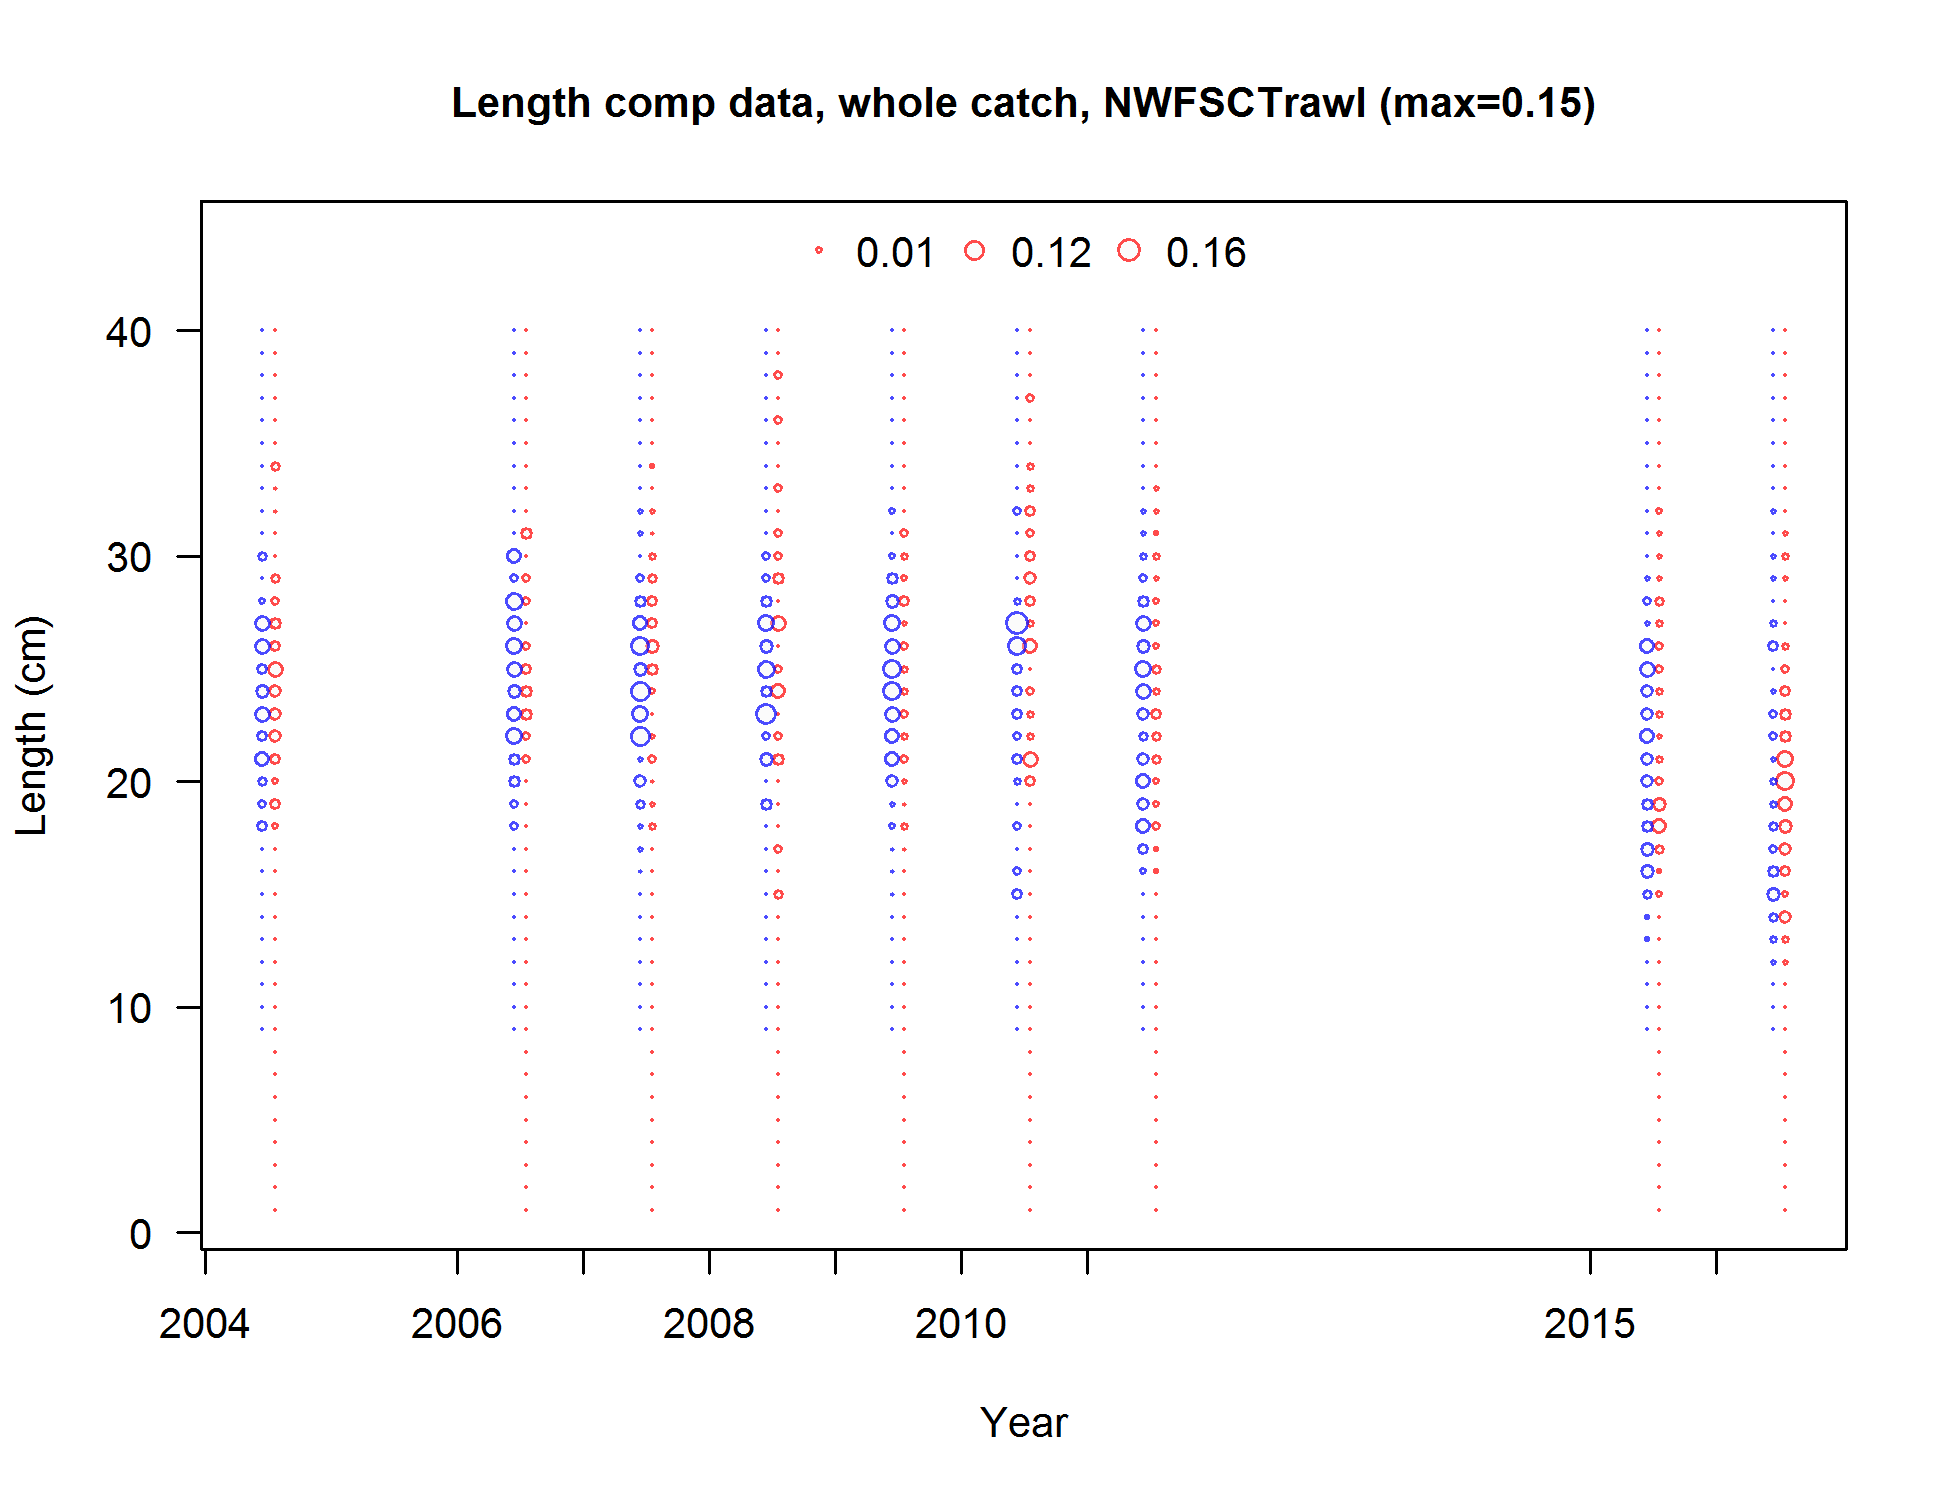
\includegraphics{r4ss/plots_mod1/comp_lendat_bubflt8mkt0.png}

\endcol
\endcols

\end{frame}

\subsection{Maturity and Fecundity}\label{maturity-and-fecundity}

\begin{itemize}
\item
  Only information on maturity from Love et al. (1987)
\item
  Found over 50\% of females were mature by 18 cm TL, or two years of
  age.
\item
  All fish were mature by 22 cm TL
\item
  No information available on fecundity of California scorpionfish
\end{itemize}

\subsection{Weight-at-length}\label{weight-at-length}

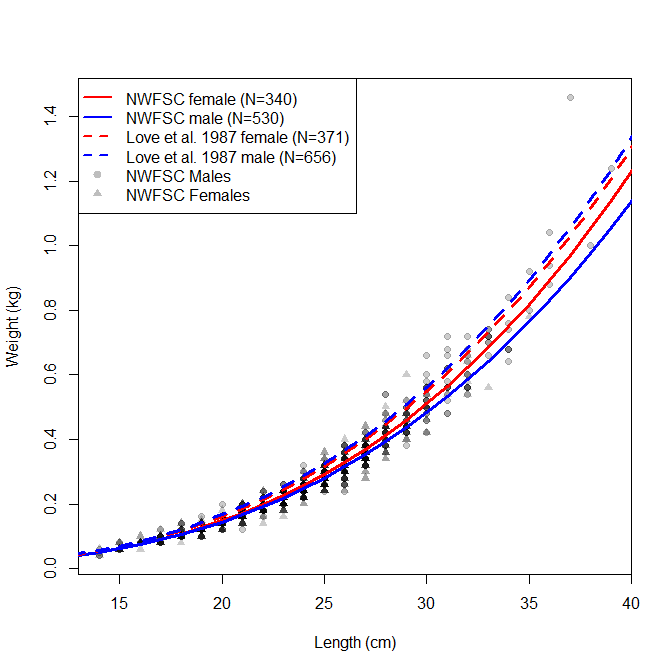
\includegraphics{Figures/Length_weight.png}

\subsection{Natural mortality}\label{natural-mortality}

\begin{itemize}
\tightlist
\item
  Prior based on maximum age of 21
\item
  Lognormal distribution with a median of 0.2715
\item
  Base model fixes female natural mortality (\(M\))
\item
  Male \(M\) estiamted as offset from female \(M\)
\item
  Sensitivities explore estimating \(M\)
\end{itemize}

\subsection{Steepness: Density-Dependent Recruitment
Compensation}\label{steepness-density-dependent-recruitment-compensation}

\begin{itemize}
\tightlist
\item
  Predictive distribution for Pacific rockfish meta-analysis
\item
  Preior mediant in 2017 for steepness (\(h\)) = 0.718
\end{itemize}

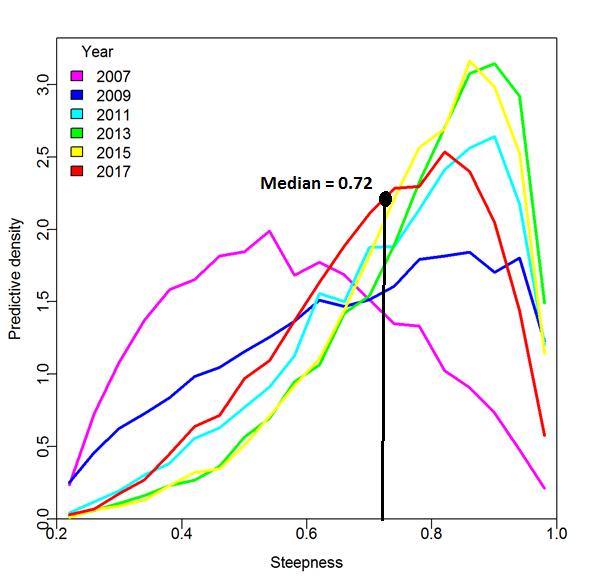
\includegraphics{Figures/h_prior.png}

\section{Removals}\label{removals}

\subsection{Total Removals}\label{total-removals}

\includegraphics{California_scorpionfish_2017_files/figure-latex/unnamed-chunk-16-1.pdf}

\subsection{Total Removals}\label{total-removals-1}

\includegraphics{California_scorpionfish_2017_files/figure-latex/unnamed-chunk-17-1.pdf}

\subsection{Total Removals}\label{total-removals-2}

\includegraphics{California_scorpionfish_2017_files/figure-latex/unnamed-chunk-18-1.pdf}

\subsection{Commercial Landings by
Fleet}\label{commercial-landings-by-fleet}

\subsection{Recreational Landings by
Fleet}\label{recreational-landings-by-fleet}

\section{Index Data}\label{index-data}

\subsection{Summary of Data Sources}\label{summary-of-data-sources}

\begin{itemize}
\tightlist
\item
  All of the methods used to standardize indices have been endorsed by
  the SSC
\end{itemize}

\begin{table}[ht]
\centering
\scalebox{0.7}{
\begin{tabular}{p{2.5in}p{0.8in}p{.4in}p{2in}}
  \hline
Name & Years & Fishery ind. & Method \\ 
  \hline
Recreational PR dockside CPUE & 2004-2016 & No & delta-GLM (bin-lognormal) \\ 
  CPFV logbook CPUE & 1980-2016 & No & negative binomial \\ 
  Onboard observer discard catch CPUE & 2002-2016 & No & delta-GLM (bin-lognormal) \\ 
  Sanitation district CPUE & 1970-2016 & Yes & delta-GLM (bin-lognormal) \\ 
  NWFSC trawl survey CPUE & 2003-2016 & Yes & VAST \\ 
  CSUN/VRG Gillnet survey CPUE & 1995-2008 & Yes & delta-GLM (bin-lognormal) \\ 
  Southern Califrnia Bight trawl survey CPUE & '94, '98, '03, '08, '13 & Yes & delta-GLM (bin-lognormal) \\ 
  Onboard observer retained catch CPUE & 2002-2016 & No & delta-GLM (bin-lognormal) \\ 
   \hline
\end{tabular}
}
\end{table}

\subsection{Recreational Private Boat
Index}\label{recreational-private-boat-index}

\subsection{Recreational Party/Charter Boat Index
(Logbook)}\label{recreational-partycharter-boat-index-logbook}

\subsection{Recreational Dead Discard
Index}\label{recreational-dead-discard-index}

\subsection{Recreational Party/Charter Retained Catch
Index}\label{recreational-partycharter-retained-catch-index}

\subsection{Sanitation Districts Survey
Index}\label{sanitation-districts-survey-index}

\begin{table}[ht]
\centering
\scalebox{0.9}{
\begin{tabular}{lrrrrr}
  \hline
Program & 0-24 m & 25-49 m & 50-74m & 100+ m & Total \\ 
  \hline
City of Los Angeles & 120 &   0 & 1372 &   0 & 1492 \\ 
  Los Angeles County & 687 &   0 & 5879 & 450 & 7016 \\ 
  Orange County & 161 & 669 & 2157 &  48 & 3035 \\ 
  City of San Diego &   0 & 404 & 333 & 829 & 1566 \\ 
   \hline
\end{tabular}
}
\end{table}

\subsection{Sanitation Districts Survey
Index}\label{sanitation-districts-survey-index-1}

\subsection{Sanitation Districts Survey
Index}\label{sanitation-districts-survey-index-2}

\subsection{NWFSC Trawl Survey Index}\label{nwfsc-trawl-survey-index}

\subsection{Gillnet Survey Index}\label{gillnet-survey-index}

\subsection{Southern California Bight Trawl Survey
Index}\label{southern-california-bight-trawl-survey-index}

\section{Composition Data}\label{composition-data}

\subsection{Dat1}\label{dat1}

\subsection{Summary of Data used in the 2017
Assessment}\label{summary-of-data-used-in-the-2017-assessment}

\end{document}
